
\chapter{Conceitos iniciais}
\label{chap:conceitos_iniciais}

	\section{Vulnerabilidade/Exploit}
	\label{sec:vuln_exploit}
	O primeiro termo que devemos definir neste trabalho é \textsl{exploit}. Mas antes dele,
	trataremos de vulnerabilidade - pois eles têm uma ligação estreita.
	Podemos definir vulnerabilidade como uma falha em um sistema que permite
	a um atacante usá-lo de uma forma não prevista pelo projetista \cite{Anley2007}.
	Ou seja, uma vulnerabilidade implica a possibilidade de uso indevido de um sistema.
	Os passos necessários para explorar essa fraqueza, ou mesmo o código (programa) que pode tirar
	proveito da vulnerabilidade é descrito como \textsl{exploit}.
	Um \textsl{exploit} surge apenas quando há uma vulnerabilidade - mas podem existir
	vulnerabilidades para as quais não exista \textsl{exploit}.

	De maneira simplificada, podemos dizer que vulnerabilidades surgem devido a 3 causas básicas:
	\begin{itemize}
		\item{Erros de implementação}
		\item{Falhas de \textsl{design}}
		\item{Erros de configuração ou de infra-estrutura do sistema}
	\end{itemize}


	\section{Conceitos básicos}
		Neste trabalho iremos tratar de \textsl{exploit}s na arquitetura x86 de 32 bits. 
		Trata-se da arquitetura de computadores
		pessoais mais difundida nos dias de hoje. Mas boa parte do estudo realizado pode ser aplicada
		a praticamente qualquer outra arquitetura.

	\section{Memória Virtual}
		Para facilitar o entendimento de questões discutidas nesse trabalho, é importante esclarecer
		pontos básicos sobre uso do esquema de memória virtual na arquitetura x86.
		Isso nos permitirá entender melhor as alternativas existentes para a implementações
		do sistemas bem como as relações com as vulnerabilidades e \textsl{exploits}.
		Primeiro repassamos as motivações e o funcionamento básico da memória virtual.
		Entre suas vantagens, conforme \cite{Bovet2005}, encontramos:
		\begin{itemize}
			\item{É possível executar aplicações que necessitam mais memória que a disponível fisicamente}
			\item{Processos podem compartilhar uma única imagem na memória de uma biblioteca}
			\item{As aplicações podem ser realocadas na memória física em qualquer lugar}
			\item{Um processo pode ser executado com apenas parte de seu código carregado em memória física}
			\item{Cada processo tem a disposição seu próprio espaço de endereçamento como se fosse
			a única aplicação no sistema} 
		\end{itemize}
		De forma geral, podemos que dizer que há um melhor uso dos recursos disponíveis e a abstração
		criada pela virtualização pode diminuir a preocupação dos programadores sobre
		como o processo é organizado na memória física.

		
		A figura \ref{fig:memoria_virtual} apresenta uma visão global do funcionamento da memória virtual.
		Nela, é mostrado como um processo pode possuir regiões diferentes de memória mapeadas
		arbitrariamente para memória física; nesse caso composta de memória RAM e de um disco de armazenamento.
		\begin{figure}
			\begin{center}
				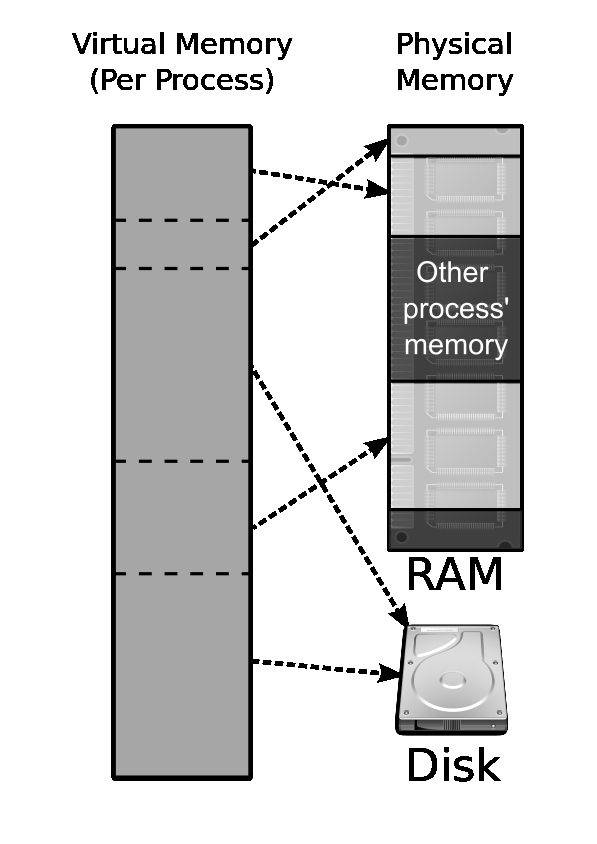
\includegraphics[width=0.35\textwidth]{Virtual_memory.jpg}
				\caption{Esquema de memória virtual (retirada da Wikepedia)}
				\label{fig:memoria_virtual}
			\end{center}
		\end{figure}
		

		\subsection{Como é usada na arquitetura x86}		
			Na arquitetura x86, a virtualização da memória é implementada com segmentação e paginação.
			Na segmentação, a memória é dividida em segmentos de tamanho variável; sendo o endereço
			virtual um identificador de segmento e um \textsl{offset}. No caso da paginação,
			a divisão da memória é feita em páginas de tamanho fixo e, analogamente, o endereço
			virtual é composto de um identificador para a página e um \textsl{offset}.
			Os dois modelos não são excludentes bem como podem ser usados independentemente.
			Nesse caso, foi optado pela presença de ambos. Assim, é possível dividir 
			a memória em segmentos que por sua vez podem ser particionados em diferentes páginas.
			
			
			Chamamos de endereço lógico aquele acessado pela aplicação - que seria, portanto
			o nível mais alto na virtualização. Já o endereço linear, é resultado do processamento
			da segmentação quando é fornecido um endereço lógico.
			Para produzir o endereço físico, ainda é necessário que a unidade de paginação
			processe o endereço linear. A figura \ref{fig:x86_end_virtual_para_fisico} ilustra esse processo.

			\begin{figure}
				\begin{center}
					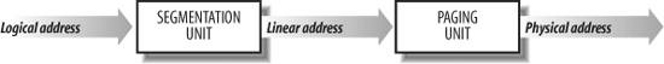
\includegraphics[width=0.8\textwidth]{x86_end_virtual_para_fisico.jpg}
					\caption{Processamento de endereço na arquitetura x86 - retirada de \cite{Bovet2005}}
					\label{fig:x86_end_virtual_para_fisico}
				\end{center}
			\end{figure}
			
			
			Assim, máquinas x86 possuem 2 níveis, segmentação e paginação na ordem, 
			a serem tratados para que um endereço físico possa ser encontrado a partir de um endereço lógico. 
			Cada um dos processos possui suas particularidades e implementa suas 
			próprias proteções conforme passamos mais detalhes a seguir.
		
		
		\subsection{Segmentação}
			Para a segmentação, a memória é organizada em segmentos e cada um deles possui diferentes atributos.
			Os principais segmentos são: o de código(mantido no registrador cs), o de dados(no registrador ds)
			e o da pilha(no registrador ss). Para os fins desse trabalho, cabe destacar os seguintes atributos
			de segmentos:
			\begin{description}
				\item[Base]
					Endereço linear inicial do segmento.
				\item[Limite]
					Endereço linear final do segmento.
				\item[Tipo]
					Os tipos definem as propriedades de acesso como leitura, escrita e execução.
				\item[DPL]
					\textsl{Descriptor Privelege Level}. Define o privilégio mínimo da CPU para
					que ele possa ser acessado. O máximo privilégio é identificado pelo valor 0;
					o menor em 3. Normalmente o sistema operacional se reserva o DPL 0, enquanto
					os demais processos ficam com 3.
			\end{description}
			Naturalmente, podem existir segmentos distintos para o sistema operacional e
			para as aplicações do usuário. Assim, aqueles pertencentes ao sistema ficam
			com DPL em zero, enquanto os demais ficam marcados como 3.


		\subsection{Paginação}
			Separando a memória em páginas de um tamanho fixo (normalmente 4Kb), 
			a paginação opera criando um mapeamento
			entre aquelas existentes na memória física e aquelas do espaço de endereçamento
			das aplicações. Assim, endereços contíguos dentro do endereço linear são mapeados
			para endereços contínuos dentro da página física.

	
			Através das tabelas de páginas, é realizado esse mapeamento. São estruturas de dados
			mantidas pelo sistema operacional com o suporte do hardware. Elas mantém
			os dados referentes às páginas. Devemos destacar as seguintes propriedades:
			\begin{description}
				\item[Leitura/Escrita]
					Indica se a página possui permissão de leitra e/ou escrita.
				\item[\textsl{User/Supervisor flag}]
					De forma análoga ao DPL na segmentação, define o privilégio mínimo exigido
					para o acesso.
			\end{description}

			
			Ao ocorrer algum problema no acesso a alguma página, como falta de privilégios
			ou mesmo porque uma página não está mapeada fisicamente, o sistema operacional
			é chamado através de uma interrupção de hardware. Dessa forma, ele pode
			tomar as medidas necessárias como: cancelar a aplicação que realizou um acesso
			ilegítimo ou buscar fazer o mapeamento da página que falta à aplicação.
			Com a cooperação do hardware e do sistema, fica possível implantar a memória
			virtual com paginação.
			

		\subsection{Caso abordado: memória virtual no sistema Linux x86} 
		\label{subsec:memoria_virtual_linux_x86}
			Conforme veremos na seção \ref{subsec:linux_kernel_vuln}, a escolha no uso da
			memória virtual no sistema Linux trouxe impactos sobre sua segurança.
			Nesse sistema, o uso da segmentação é extremamente limitado.
			A paginação foi escolhida em detrimento à segmentação - sendo a última
			usada apenas por obrigatoriedade da arquitetura.
			Os segmentos de dados e código para o sistema operacional e para as aplicações do
			usuário são praticamente os mesmos. A tabela \ref{tab:descritores_segmentos_linux}
			apresenta os principais segmentos.


			Embora isso tenha vantagens em termos de desempenho, pois facilita a troca
			de contexto entre modo usuário e modo do sistema bem como a troca de dados
			entre ambos, há uma desvantagem de segurança.
			\begin{table}
				\begin{tabular}{|l|c|c|c|c|}
					\hline
						\textbf{Segmento} & \textbf{Base} & \textbf{Limite} & \textbf{Tipo} & \textbf{DPL}\\
					\hline
						Código do usuário & 0x00000000 & 0xfffff & Leitura & 3\\
					\hline
						Dados do usuário & 0x00000000 & 0xfffff & Escrita/Leitura &	3\\
					\hline
						Código do kernel & 0x00000000 & 0xfffff & Leitura &	0\\
					\hline
						Dados do kernel & 0x00000000 & 0xfffff & Escrita/Leitura &	0\\
					\hline
				\end{tabular}
				\caption{Quatro segmentos principais no Linux com seus descritores}\label{tab:descritores_segmentos_linux}
			\end{table}
			Tanto o kernel as aplicações do usuário podem usar os mesmos endereços lógicos.
			Certas restrições de segurança acabam recaindo, portanto, apenas para a paginação.
			

	\section{Gerência de memória}
	\label{sec:gerencia_memoria}
	O controle da memória é um ponto crítico. Falhas nele acabam resultando em vulnerabilidades 
	gravíssimas. Faremos uma breve abordagem sobre o gerenciamento de memória sobre
	o ponto de vista dos \textsl{exploit}s.

	Um primeiro ponto a destacar sobre a memória é um princípio básico que norteia
	quase todas as arquiteturas modernas. Dados e instruções não são diferenciados na memória.
	Ou seja, não há uma separação rígida entre instruções que compõem um programa e os dados
	sobre os quais opera. Essa característica foi herdada da arquitetura básica de von Neumann.
	Como veremos a seguir, essa decisão de design, com origem nos anos 1940, embora tenha
	facilitado a evolução dos computadores, abriu caminhos para os \textsl{exploit}s que conhecemos hoje. 

	Abaixo descrevemos o layout básico da memória de um processo em um sistema UNIX.
	Ele pode ser separado em 6 partes fundamentais:
	\begin{description}
		\item[text]
			A parte que contém as instruções do programa - seu código propriamente dito.
			Seu tamanho é fixo durante a execução e ela não deve possibilitar escrita.
		\item[data]
			Contém variáveis globais já inicializadas. Seu tamanho é fixo durante a execução.
		\item[bss]
			Nome de origem história significando Block Started by Symbol. Área da memória responsável
			por armazenar variáveis globais	não inicializadas. Como text e data, bss também tem tamanho 
			fixo conhecido desde o início do processo. 
		\item[Heap]
			Espaço para variáveis alocadas dinamicamente. A chamada de sistema sbrk é responsável
			pelo controle do crescimento/encolhimento desse espaço. Bibliotecas geralmente facilitam a vida
			do programador disponibilizando interfaces mais amigáveis como malloc() e free(). Assim a biblioteca
			se encarrega de chamar sbrk() para diminuir/aumentar o Heap. Ela cresce do endereço mais baixo para o
			mais alto.
		\item[Stack]
			Mantém controle das chamadas de funções. Possibilita a recursividade. Logo, possui
			tamanho variável - crescendo do endereço mais alto para o mais baixo (sendo antagonista do Heap - ver
			figura \ref{fig:regioes_memoria}). 
			Esse crescimento é que torna possível que uma chamada de função que tenha seus dados
			sobrescritos influencie numa chamada de função anterior. Esse é o princípio do buffer overflow - tratado
			posteriormente.
		\item[Enviroment]
			A última porção de memória do processo guarda uma cópia das variáveis de ambiente do sistema.
			Essa seção possui permissão de escrita, mas como bss, data e text, possui tamanho fixo.
	\end{description}

	\begin{figure}
		\begin{center}
		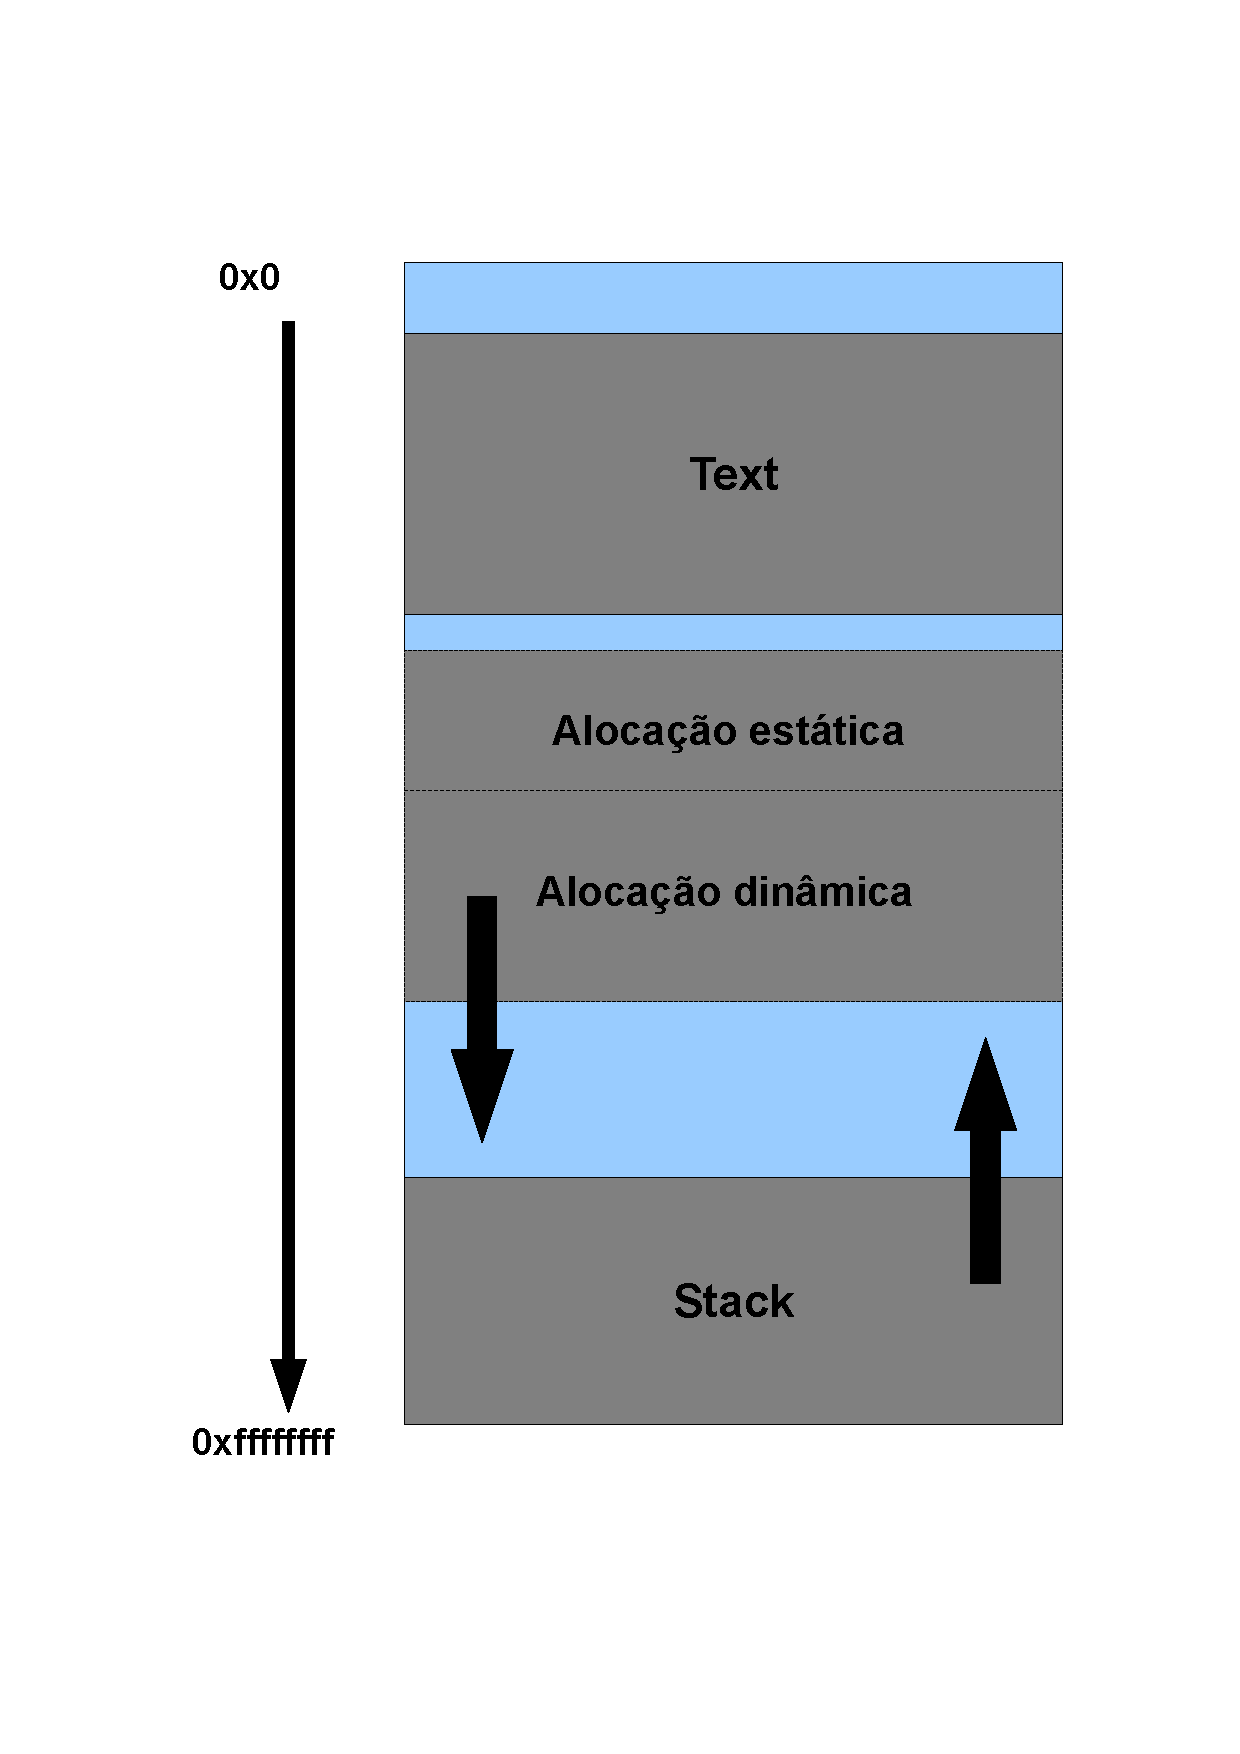
\includegraphics[width=0.45\textwidth]{regioes_memoria.pdf}
		\caption{Regiões de memória em um processo.}
		\label{fig:regioes_memoria}
		\end{center}
	\end{figure}

	\section{Funcionamento mais detalhado do Stack}
	A pilha é uma região contínua com base fixa e tamanho variável.
	Na arquitetura abordada por esse trabalho, x86 (bem como em muitas outras), a pilha cresce
	em direção ao endereço mais baixo. É organizada em \textsl{frames} que são os blocos
	alocados quando ocorrem chamadas a funções. Cada \textsl{frame} contém(ver figura \ref{fig:stack_frame}):
	\begin{itemize}
		\item parâmetros
		\item variáveis locais
		\item endereço de retorno da função anterior
		\item endereço do \textsl{frame} da função que a chamou
	\end{itemize}

	\begin{figure}
		\begin{center}
		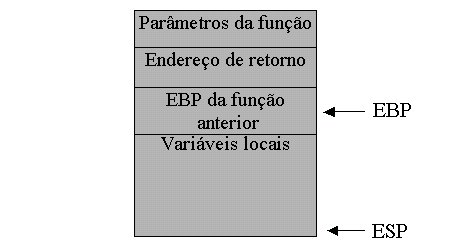
\includegraphics[width=0.5\textwidth]{stack_frame_furlan.jpg}
		\caption{Organização do \textsl{frame} na pilha. Retirado de \cite{Furlan2005} pg. 17.}
		\label{fig:stack_frame}
		\end{center}
	\end{figure}

	\subsection{Chamada de funções}
	Quando uma função é chamada, seus parâmetros são empilhadas e posteriormente o endereço
	do retorno. Isso fica a encargo da função que faz a chamada.
	Para completar o \textsl{frame}, aquela que é chamada, empilha o endereço do frame da função chamadora
	(EBP) e posteriormente aloca na pilha o espaço correspondente a suas variáveis locais.
	É importante ressaltar que, caso o endereço de retorno, empilhado por quem chama, seja alterado,
	o fluxo de execução é mudado. Pois é justamente este o princípio do \textsl{buffer overflow}.
	Ele será abordado em maior detalhes na Seção \ref{subsec:buffer_overflow}.

	\section{Funcionamento mais detalhado do Heap}
	\label{sec:funcionamento_heap}
	A porção de memória correspondente ao heap possibilita ao programador alocar dinamicamente memória
	que fica disponível durante toda a execução para qualquer chamada de função.
	Existem diversas formas de administrar a memória do heap, mas o mais encontrado, conforme
	\cite{Love2007}, é dividir o todo em partições de potências de 2. Chamadas à função malloc()/free(),
	em última análise, correspondem a operações de alocar/liberar partições internas do heap.
	Normalmente a organização das partições se dá como forma de uma lista encadeada.
	Assim, para efetuar o controle dos blocos, são mantidas meta-informações que determinam
	tamanho, endereço do próximo bloco livre - entre outros - para que a gerência
	da memória dinâmica seja eficiente.
	Uma chamada a free(), por exemplo, pode implicar acerto de diversos ponteiros que existem
	dentro das partições no heap.
	 

	Havendo uma validação incorreta no software, pode ocorrer um \textsl{overflow} na área do
	heap. Se os dados escritos sobrepuserem os valores dos ponteiros de controle interno dos blocos,
	fica aberto um caminho para que um atacante consiga uma escrita em um endereço arbitrário.
	Pois é esse o princípio básico de funcionamento de \textsl{Heap Overflow}. Ele pressupõe
	o conhecimento aprofundado da gerência do heap; pois só dessa forma é possível prever
	exatamente como os blocos são mantidos.

	\section{Mapemamento de memória anônimo}
	Como visto no funcionamento básico do Heap, a fragmentação é um problema a ser considerado.
	Uma forma alternativa de alocar memória dinamicamente que não usa o Heap são os mapeamentos anônimos.
	No Linux por exemplo, através da função mmap() é possível alocar um bloco de memória contínuo
	fora do Heap que não está sujeito aos problemas de fragmentação.
	Conforme, \cite{Love2007}, é possível considerar esse espaço de memória como um novo Heap
	vindo de apenas uma alocação.
	No exemplo a seguir, é requisitado uma porção de memória de 64 bytes iniciando em NULL.
	\begin{verbatim}
		mmap(NULL, 64, PROT_READ | PROT_WRITE,
			MAP_FIXED | MAP_ANONYMOUS | MAP_PRIVATE, 0, 0);
	\end{verbatim}
	Na técnica \textsl{NULL pointer exploit}, conforme veremos mais adiante, essa possibilidade
	de alocarmos um bloco com o início pré-determinado é muito útil.
	No caso da chamada de mmap() do exemplo anterior, estamos obtendo um bloco de 64 bytes começando
	no endereço zero(NULL). Isso nos permite colocar código executável nessa porção da memória e,
	na presença de uma vulnerabilidade, desviar a execução para esse ponto.
	
	\section{Registradores de controle}
	Uma parte fundamental da arquitetura que deve ser mencionada são os registradores que possuem
	relação direta com o gerenciamento da memória.
	Talvez o mais importante (na arquitetura base do estudo IA32) seja o EIP(Extended Instruction Pointer).
	Ele indica o endereço da próxima instrução. Sobrescrevê-lo equivale obter o controle
	do fluxo de um processo.
	Além dele, destacamos EBP(Extended Base Pointer) e ESP(Extended Stack Pointer).
	ESP indica o endereço do último valor inserido na pilha.
	O EBP indica o início da pilha para aquela chamada de função. É usado para referenciar variáveis
	locais da função.

	\section{Shellcode}
	Outra parte fundamental de quase todo \textsl{exploit} é o chamado \textsl{shellcode}.
	Podemos definí-lo, segundo \cite{Anley2007}, como um conjunto de instruções que são injetados
	e executados por um programa através de um \textsl{exploit}. 


	A palavra \textsl{shell} contida em seu nome tem origem no fato de, normalmente, ele ser usado
	para abrir um \textsl{shell} na máquina atacada. Sendo aberto com permissões de \textsl{root},
	o atacante assume controle absoluto do sistema. Ainda que isso seja o mais comum, o \textsl{shellcode}
	não se restringe a isso. Como qualquer outro programa, ele, em muitos casos, só é limitado pela imaginação
	do seu construtor.
	
